Tout d’abord, reprenons le problème I qui est très similaire au début de la consigne. Pour chaque signal, nous devons calculer la puissance du signal avec des fenêtres glissantes. Autrement dit, nous devons calculer la puissance des n échantillons de chaque fenêtre de taille n. 
\\
Nous savons que la taille de la fenêtre glissante est $2*K + 1$ et sa durée, $D = (2*K + 1) \times Te $ (Te étant la période d’échantillonnage). 
\\
Dans le cas de signaux sonores, il est souhaitable d’avoir une durée de fenêtre de l’ordre de la seconde, ou en dessous. Nous ferons le choix arbitraire de 0.5s de durée, autrement dit, $K=\frac{\frac{0.5}{T_e}-1}{2}$. 
\\ \\
A partir de là, nous calculons les puissances de chaque fenêtre comme la valeur de chaque échantillon au carré, divisé par la taille de fenêtre. 
Une fois le tableau de puissances « fenêtrées » créé, il faut seuiller la puissance en dBm par la valeur de référence PdBm. PdBm se calcule en reprenant la formule du problème I (ou III). 
\begin{equation}
    P_{dBm} = 20\log(S_{REF}*10^\frac{S}{20}*P_{REF}*10^\frac{P_{SPL}}{20}*10^\frac{G}{20})
\end{equation}
En simplifiant, nous obtenons : 
\begin{equation}
    P_{dBm} = 20\log(S_{REF}) + S + 20\log(P_{REF}) + P_{SPL} + G + 30
\end{equation}
D’où :
\begin{equation}
    P_{dBm} = G + S + P_{SPL} + 30 + 20\times \log(20\times10^{-6}) = -5
\end{equation}

Une fois cela fait et appliqué aux signaux qui nous ont été donnés, nous obtenons les figures suivantes \ref{Fig.sub.4.2.1}, \ref{Fig.sub.4.2.2}, \ref{Fig.sub.4.2.3}, \ref{Fig.sub.4.2.4}. Les pointillés \textcolor{red}{rouges} au niveau des figures représentent le seuil à -5 dBm.

\begin{figure}[htb]
\subfigure[Puissance en dBm et seuil sur le signal Alarme]{
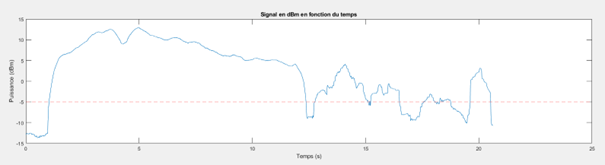
\includegraphics[width = 0.45\textwidth]{puissance alarme dbm.png}
\label{Fig.sub.4.2.1}
}
\subfigure[Puissance en dBm et seuil sur le signal Jardin01]{
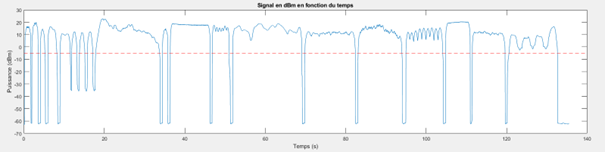
\includegraphics[width = 0.45\textwidth]{puissance jardin01 dbm.png}
\label{Fig.sub.4.2.2}
}
\subfigure[Puissance en dBm et seuil sur le signal MarteauPiqueur]{
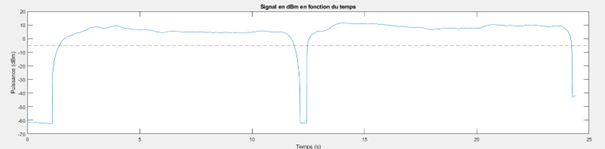
\includegraphics[width = 0.45\textwidth]{puissance marteauPiqueur dbm.png}
\label{Fig.sub.4.2.3}
}
\subfigure[Puissance en dBm et seuil sur le signal Ville01]{
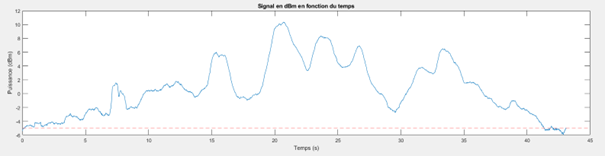
\includegraphics[width = 0.45\textwidth]{puissance ville01 dbm.png}
\label{Fig.sub.4.2.4}
}
\caption{Puissance en dBm (avec seuil à -5 $P_{dBm}$)}
\label{Fig.main.2}
\end{figure}
Ensuite, nous détectons les plages de ces signaux, qui durent plus d’une seconde et dépassent la valeur seuil, puis nous les colorons en \textcolor{red}{rouge}, le reste du signal est en \textcolor{blue}{bleu}.
